
% !TEX encoding = UTF-8 Unicode
\documentclass[12pt]{article}
\usepackage[english,greek]{babel}
\usepackage[utf8x]{inputenc}
\usepackage{amssymb,latexsym,amsmath,ucs,amsthm,setspace,graphicx}
\usepackage{kerkis}
\usepackage{tikz}
\usepackage{algorithm2e}

\newcommand{\HRule}{\rule{\linewidth}{0.5mm}}


\begin{document}
\begin{titlepage}
\centering


\includegraphics[scale=0.3]{pyrforos.jpg}

\textsc{\LARGE Σχολή \\ Ηλεκτρολόγων Μηχανικών \\[-3pt] και \\[6pt] Μηχανικών Υπολογιστών}

\vspace{1cm}

% Title
\HRule \\[0.4cm]
{\huge \bfseries Λειτουργικά Συστήματα\\} %\\

\vspace{0.4cm}
\HRule \\[0.4cm]

\Large{3η σειρά ασκήσεων\\}


% Authors
\vfill
\begin{center}
\large
%Add authors one after another with the same format
\textlatin{oslabb12}

Γκούμας Βασίλης ---  03113031 

Ζαρίφης Νικόλαος --- 03112178

%\vfill
\end{center}

\end{titlepage}

\section*{Άσκηση 1}
Ο κώδικας της άσκησης βρίσκεται στο αρχείο \textlatin{simplesync.c}

Στόχος της άσκησης είναι ο συγχρονισμός δύο νημάτων εκτέλεσης, ένα που αυξάνει τη τιμή μιας μοιραζόμενης μεταβλητής και ένα που την μειώνει, ώστε μετά το πέρας της εκτέλεσης των νημάτων να πάρουμε τα σωστά αποτελέσματα. \\
Αυτό ζητείται να υλοποιηθεί με δύο τρόπους, με \textlatin{atomic operations} και \textlatin{mutex locks}. 

\subsection*{Ερωτήματα 1-2}Μελετώντας το \textlatin{Makefile} που μας δίνεται, βλέπουμε πως απο το ίδιο αρχείο κώδικα ( \textlatin{simplesync.c} ) παράγονται δύο εκτελέσιμα, τα \textlatin{simplesync-atomic} και \textlatin{simplesync-mutex}.  
Αυτό πετυχαίνεται μέσω των \textlatin{\#define macros} που υπάρχουν στον κώδικα.
 Συγκεκριμένα κατά το \textlatin{compilation}, στη μία παραλλαγή του εκτελέσιμου περνάμε την παράμετρο \textlatin{DSYNC\_MUTEX}, η οποία συμπεριλαμβάνει τα κομμάτια κώδικα που βρίσκονται μέσα στα τμήματα \textlatin{\#ifdefine SYNC\_MUTEX}.
 
'Οσον αφορά το χρόνο εκτέλεσης των δύο προγραμμάτων έχουμε τα παρακάτω \textlatin{"benchmark"}:

\begin{itemize}

\item \textlatin{simplesync}: \\
\textlatin{
real	0m0.044s    \\
user	0m0.036s    \\
sys	0m0.000s    \\
}

\item \textlatin{simplesync-atomic}:  \\
\textlatin{
real	0m0.140s \\
user	0m0.132s \\
sys	0m0.000s \\
}
								
\item \textlatin{simplesync-mutex}:  \\
\textlatin{
real	0m0.767s \\
user	0m0.764s \\
sys	0m0.000s \\
}

\end{itemize}

Βλέπουμε λοιπόν πως ταχύτερο είναι το εκτελέσιμο χωρίς συγχρονισμό, ακολουθεί το \textlatin{simplesync-atomic} και τέλος το \textlatin{simplesync-mutex}.
Η παραπάνω διαφορά στον χρόνο εκτέλεσης, οφείλεται στο ότι το \textlatin{simplesync-atomic} υλοποιείται με \textlatin{atomic operations}, οι οποίες μεταφράζονται σε \textbf{μία} ( κατα προσέγγιση )εντολή \textlatin{assembly}. Απο την άλλη, η έννοια των \textlatin{mutex} αποτελεί μια πιο \textlatin{high level} ιδεά και ενσωματώνει την έννοια των \textlatin{atomic operations} για να υλοποιηθεί. Τέλος, το ασυγχρόνιστο εκτελέσιμο είναι το γρηγορότερο καθώς δε χρειάζεται να ασκηθεί κάποιος περιορισμός στην εκτέλεση των δύο \textlatin{threads} . \\

Παρακάτω βλέπουμε το αποτέλεσμα της εκτέλεσης των τριών παραπάνω προγραμμάτων.


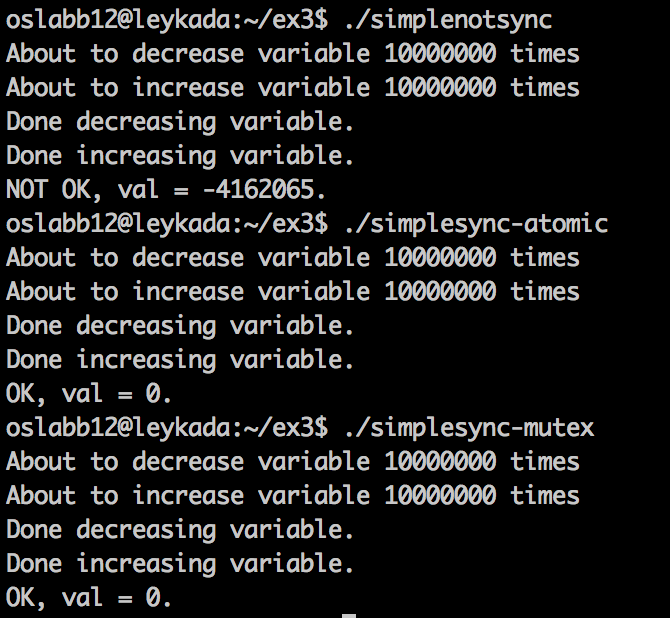
\includegraphics[scale=0.5]{ask3-sync.png}

\subsection*{Ερώτημα 3}
Παρακάτω βλέπουμε τις εντολές \textlatin{assembly} στις οποίες μεταγλωττίζεται η \textlatin{sync\_fetch\_and\_sub}. Για την αντίστοιχη \textlatin{add} απλά λείπουν οι εντολές που εκτελούν την αντιστροφή στην αριθμητική συμπληρώματος ως προς δύο. Έχουμε:\\ 

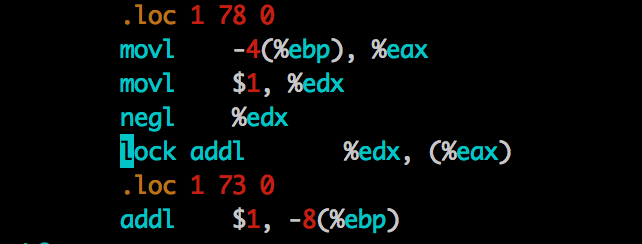
\includegraphics[scale=0.5]{ask3-atomic.png}

Μετά τον κώδικα διαχείρισης της στοίβας ( δημιουργία του \textlatin{stack frame} ) για την κλήση της συνάρτησης, έχουμε την κύρια λειτουργία της \textlatin{atomic} λειτουργίας, που υλοποιείται με την εντολή \textlatin{lock addl}.

\subsection*{Ερώτημα 4}
Ο αντίστοιχος κώδικας \textlatin{assembly} που παράγεται για την \textlatin{pthread\_mutex\_lock()} φαίνεται παρακάτω: \\
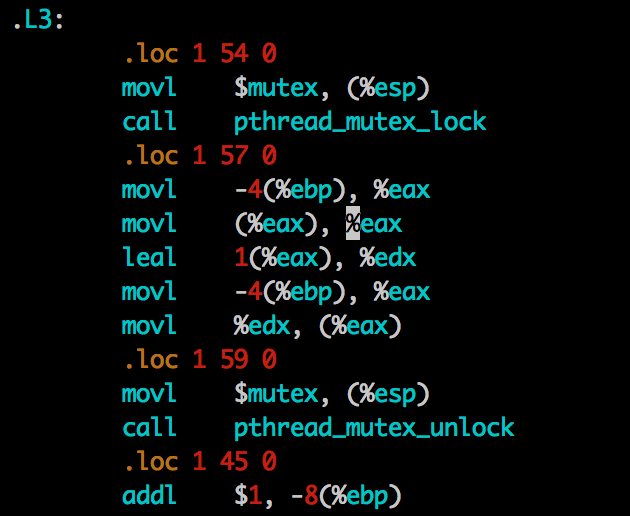
\includegraphics[scale=0.5]{ask3-mutex.png}


\section*{Άσκηση 2}

Ο κώδικας της άσκησης βρίσκεται στο αρχείο \textlatin{mande.c}

\subsection*{Ερώτημα 1}
Στο πρόγραμμά μας χρειάστηκαν συνολικά $N$ σημαφόροι, ένας για κάθε \textlatin{thread}. Συγκεκριμένα για κάθε νήμα, ο σημαφόρος του ενεργοποιείται με τη λήξη της εργασίας του $N-1$ νήματος και με την ολοκλήρωση του σηματοδοτεί την έναρξη του $N+1$ νήματος. Αναλυτικότερα το σχήμα συγχρονισμού μας λειτουργεί σαν κυκλικός δακτύλιος, με το κάθε νήμα να παίρνει την άδεια προς εκτέλεση απο το προηγούμενό του και την άδεια  $0$.


\subsection*{Ερώτημα 2}
Σε διπύρηνο μηχάνημα χρονομετρήσαμε την εκτέλεση των δύο προγραμμάτων και έχουμε: \\

\begin{itemize}

\item σειριακή εκδοχή \\ 
\textlatin{
real	0m0.778s   \\
user	0m0.776s   \\
sys	0m0.000s   \\
}

\item παράλληλη εκδοχή ( 2 νήματα ) \\
\textlatin{
real	0m0.395s \\
user	0m0.772s \\
sys	0m0.008s \\
}

\end{itemize}

\subsection*{Ερώτημα 3}
Όπως βλέπουμε απο τις παραπάνω μετρήσεις το παράλληλο πρόγραμμα εμφανίζει επιτάχυνση. Αυτο είναι λογικό, καθώς η φάση υπολογισμού γίνεται παράλληλα και ο συγχρονισμός επιστρατεύεται ώστε να γίνει με τη κατάλληλη σειρά το τύπωμα.  Σε αντίθετη περίπτωση δε θα είχαμε επιτάχυνση, καθώς το κάθε νήμα θα περίμενε το προηγούμενο για να υπολογίστει, με αποτέλεσμα το πρόγραμμα να εκφυλίζεται στο αντίστοιχο σειριακό, με πιθανώς χειρότερη επίδοση λόγω \textlatin{ context switching}.


\subsection*{Ερώτημα 4}
Με το πάτημα του \textlatin{CTRL-C} το πρόγραμμα μας τερματίζει, καθώς του στέλενται σήμα \textlatin{SIGINT}. Ως αποτέλεσμα το χρώμα των γραμμών του τερματικού παραμένει σε αυτό που είχε επιλεχθεί για τύπωμα ακριβώς πριν τον τερματισμό του προγράμματος. \\
Μια λύση είναι να υλοποιήσουμε τον δικό μας \textlatin{signal handler} που με το πάτημα του \textlatin{CTRL-C} να επαναφέρει το \textlatin{default} χρώμα και στη συνέχεια να τερματίζει.





\section*{'Ασκηση 3}

Ο κώδικας της άσκησης βρίσκεται στο αρχέιο \textlatin{kgarten.c}

Το αποτέλεσμα της εκτέλεσης για ενδεικτικές τιμές που δοκιμάζουν το σχήμα συγχρονισμού βρίσκονται στον φάκελο \textlatin{out3}.


Στην άσκηση αυτή μας ζητείται η υλοποίηση ενός σχήματος συγχρονισμού για ένα νηπιαγωγείο. Ο χρυσός κανόνας είναι ότι αν $t,c,r$ είναι το πλήθος των δασκάλων, των παιδιών και το \textlatin{ratio} που δίνεται, πρέπει κάθε στιγμή μέσα στο νηπιαγωγείο να ισχύει η σχέση:
\[ t \cdot r \geq c \]

Για την παραπάνω υλοποίηση μεταβάλλαμε μόνο τον κώδικα των συναρτήσεων \textlatin{*\_enter} και \textlatin{*\_exit}.

Στη  συνέχεια περιγράφεται  το σχήμα συγρονισμού που χρησιμοποιήθηκε. Οι κρίσιμες λειτουργίες είναι οι \textlatin{child\_enter} και η \textlatin{teacher\_exit} καθώς αυτές απαιτούν τον έλεγχο της αντίστοιχης συνθήκης πριν να είναι δυνατή η έξοδος/είσοδος. 

Αντιθέτως, οι συναρτήσεις \textlatin{child\_exit} και \textlatin{teacher\_enter} δεν έχουν κάποιο περιορισμό καθώς κάποιο παιδί μπορεί να φύγει οποιαδήποτε στιγμή ή κάποιος δάσκαλος να έρθει, χωρίς να επηρεάζουν την αλήθεια της συνθήκης. Επομένως μετά την αυξομείωση των κοινών \textlatin{resources} οι παραπάνω συναρτήσεις οφείλουν να σηματοδοτήσουν τις \textlatin{child\_enter}, \textlatin{teacher\_exit}, σε περίπτωση που ισχύει η αντίστοιχη συνθήκη.

Το παραπάνω γεγονός το αναπαριστούμε με τις \textlatin{conditional variables} με όνομα \textlatin{teacher\_out, child\_in} που σηματοδοτούνται όταν ισχύει η κατάλληλη συνθήκη.
Η σηματοδότηση γίνεται απο όλες τις συναρτήσεις, ώστε να εξαλείψουμε στο έπακρο τυχόν \textlatin{race conditions}.

Επίσης προσθέσαμε τη μεταβλητή \textlatin{count} που συμβολίζει το πλήθος των παιδιών που μπορούν να μπουν ακόμα και  απλουστεύει τον έλεγχο των συνθηκών και τέλος η πρόσβαση σε όλους τους κοινούς πόρους έγινε μέσω κλειδώματος με \textlatin{mutex}.

Εξίσου σημαντικό είναι ότι μετά απο οποιδήποτε ενέργεια ελέγχεται ξανά η συνθήκη ώστε να σηματοδοτήσει την αντίστοιχη είσοδο/έξοδο.


Το σχήμα συγχρονισμού μας είναι ορθό και εξασφαλίζει τη πρόοδο ( \textlatin{progress} ). Ορθο διότι πριν απο κάθε είσοδο παιδιού/έξοδο δασκάλου, εξασφαλίζει ότι η συνθήκη είναι είναι αληθής.Επίσης εξασφαλίζει πρόοδο γιατί κάθε ενέργεια "προωθεί" κάθε επόμενη διαθέσιμη ενέργεια, δηλαδή μετά απο κάθε έισοδο/έξοδο, ελέγχεται αν μπορεί να βγεί κάποιος δάσκαλος ή να μπεί κάποιο παιδί. \\
Έτσι αποτρέπονται τα \textbf{τεχνητά} \textlatin{race conditions}, δηλαδή απο παράβλεψη του σχήματος υλοποίησης και επομένως εμφανίζονται μόνο τα φυσικά, που εξαρτώνται απο τη σειρά με την οποία θα έρθουν τα νήματα. Το σχήμα μας είναι \textlatin{best effort} με την έννοια ότι δεν κάνει διακρίσεις στα νήματα που έρχονται και προσπαθεί να τα ικανοποιήσει όλα χωρίς να εισάγει νέα κολλήματα και είναι ευάλωτο αποκλειστικά στη σειρά και το πλήθος των νημάτων που καταφθάνουν.




\subsection*{Ερώτημα 1}

Στο σχήμα συγχρονισμού που περιγράψαμε και υλοποιήσαμε, όταν υπάρχουν παιδιά και δάσκαλοι που περιμένουν να βγουν/μπουν, τότε εξυπηρετείται τυχαία κάποιο αίτημα, ανεξαρτήτου του χρόνου αναμονής.
Για παράδειγμα ένα παιδί που μόλις έφτασε μπορεί να μπεί αμέσως, ενώ ένας δάσκαλος να περιμένει αρκετή ώρα για να βγεί. Αυτο εξαρτάται απο τη σειρά εκτέλεσης των νημάτων.

\subsection*{Ερώτημα 2}

Το παραπάνω \textlatin{race condition} εμφανίζεται και στον έλεγχο ορθότητας του \textlatin{kgarten.c} . Επομένως το πρόγραμμά μας είναι έρμαιο αποκλειστικά της τυχαιότητας καθώς όπως είδαμε η συνθήκη δε παραβιάζεται ποτέ και η υλοποιήση δε μπλοκάρει καμία είσοδο/έξοδο του νηπιαγωγείου.



\section*{'Προαιρετικές 'Ασκήσεις}

\subsection*{Ερώτημα 1}

Ένας παρακολουθητής ( \textlatin{Monitor} ) που υλοποιεί τη λειτουργία σημαφόρου θα είχε δύο μεθόδους, η πρώτη είναι η  \textlatin{wait()} που παγώνει την εκτέλεση της διεργασίας, αναμένοντας την \textlatin{signal()}.Η δεύτερη είναι η \textlatin{signal()}, που ξυπνάει κάποια διεργασία απο το σωρό νημάτων ( \textlatin{thread pool} ) 


\subsection*{Ερώτημα 2}
Το δοσμένο πρόγραμμα παίρνει προαιρετικά ως παράμετρο έναν αριθμό απο τη γραμμή εντολών και τυπώνει τόσους τυχαίους αριθμούς ( σε περίπτωση που δε δωθεί όρισμα τυπώνει 10 ). Τρέχοντας όμως το πρόγραμμα παρατηρούμε ότι δεν παίρνουμε τα αναμενόμενα αποτελέσματα, αλλα τους ίδιους αριθμούς.

 Αυτό συμβαίνει, γιατί οι \textlatin{spawned processes} που αναλαμβάνουν το τύπωμα έχουν κληρονομήσει το ίδιο \textlatin{seed}, το οποίο χρησιμοποιεί η \textlatin{rand} για τη παραγωγή "τυχαίων" αριθμών, και ως αποτέλεσμα όλες οι κλήσεις στην \textlatin{rand} θα επιστρέψουν την ίδια τιμή ( ακόμα αν είχαμε και παραπάνω απο μία τιμές για κάθε διεργασία ).
 
 Αυτό οφείλεται στο ότι η εντολή \textlatin{srand(time(NULL))} που χρησιμοποιείται ως αρχικοποίηση του  \textlatin{seed}, η τιμή του οποίου εξαρτάται απο την τρέχουσα ώρα, καλείται μια φορά στην αρχή του προγράμματος, αντί σε κάθε διεργασία ξεχωριστά, έτσι όλες οι γεννήτριες ψευδοτυχαίων αριθμών κληρονομούν το ίδιο \textlatin{seed} και άρα θα τυπώνουν ίδιους αριθμούς.
 
 \subsection*{Ερώτημα 3}
 
 Μια υλοποίηση που θα έδινε διαφορετική πιθανότητα επιλογής σε παιδιά και δασκάλους, θα ήταν η ύπαρξη δύο ουρών, μία για τους δασκάλους και μία για τα παιδιά.

 Επομένως κάθε φορά που επιλέγεται νήμα προς εκτέλεση θα επιλέγεται με μεγαλύτερη πιθανότητα η ουρά με τα νήματα παιδιών.

\end{document}

